\section{Review of vector algebra}

	\subsection{Addition of vectors}
		Two or more vectors may be added by geometrical laws, which are discussed below:
		
		\begin{enumerate}
			\item \textit{Triangle law of vector addition}
			
			\textit{\ul{Statement}}: If two vectors are represented both in magnitude and direction by two sides of a triangle taken in the \textit{same order}, then their resultant vector is represented both in magnitude and direction by the third side of the triangle taken in the \textit{opposite order}.
			
			\textbf{Note}: Vectors are in the \textit{same order} when one's origin coincides with the other's terminus; otherwise, they are in the \textit{opposite order}.
			
%				\textit{\ul{Demonstration}}:
%				\begin{enumerate}[I.]
%					\item Suppose there are two vectors $\va*{A}$ and $\va*{B}$ which are to be added. In general, they may lie anywhere with respect to each other.
%					
%					\item Then we displace either of the vectors parallel to itself and place it such that its origin coincides with the terminus of the other vector (or vice versa).
%					
%					\item The resultant vector sum $\va*{A}+\va*{B}=\va*{B}+\va*{A}$ is a vector pointing from the non-coinciding origin to terminus.
%				\end{enumerate}
			
			\item \textit{Parallelogram law of vector addition}
			
			\textit{\ul{Statement}}: If two vectors acting at the same point are represented both in magnitude and direction by the adjacent sides of a parallelogram, then their resultant is represented both in magnitude and direction by the diagonal of that parallelogram passing through the same point.
			
%				\textit{\ul{Demonstration}}:
%				\begin{enumerate}[I.]
%					\item Suppose there are two vectors $\va*{A}$ and $\va*{B}$ which are to be added. Here as well, in general, they may lie anywhere with respect to each other.
%					
%					\item Then we displace either of the vectors parallel to itself and place it such that their origins coincide.
%					
%					\item We complete the parallelogram by drawing two line segments parallel to $\va*{A}$ and $\va*{B}$ from their respective termini.
%					
%					\item The resultant vector sum $\va*{R}=\va*{A}+\va*{B}$ is the vector along the \textit{main diagonal} of the parallelogram, i.e. the one whose origin also coincides with the common origins of $\va*{A}$ and $\va*{B}$.
%				\end{enumerate}
			
			\item \textit{Polygon law of vector addition}
			
			\textit{\ul{Statement}}: If several vectors are represented both in magnitude and direction by the sides of a polygon taken in order, then their resultant is represented both in magnitude and direction by the closing side taken in reverse order.
			
%				\textit{\ul{Demonstration}}:
%				\begin{enumerate}[I.]
%					\item Suppose there are four vectors $\va*{A}$, $\va*{B}$, $\va*{C}$ and $\va*{D}$ which are to be added.
%					
%					\item Then we rearrange the vectors in such a way that they are in order, thereby forming the sides of a polygon, except for the closing side.
%					
%					\item The resultant vector sum $\va*{R}=\va*{A}+\va*{B}+\va*{C}+\va*{D}$ is the vector along the closing side of the polygon taken in the opposite order.
%				\end{enumerate}
		\end{enumerate}
		
		\subsubsection{Properties of vector addition}
			\begin{enumerate}[i.]
				\item Vector addition is \textit{commutative}, i.e.
				$$\va*{A}+\va*{B}=\va*{B}+\va*{A}$$
				
				\item Vector addition is \textit{associative}, i.e.
				$$\va*{A}+\qty(\va*{B}+\va*{C})=\qty(\va*{A}+\va*{B})+\va*{C}$$
				
				\item Vector addition is \textit{distributive}, i.e.
				$$\lambda\qty(\va*{A}+\va*{B})=\lambda\va*{A}+\lambda\va*{B}$$
				where $\lambda$ is a real number.
				
				\item The sum of two negative vectors is a null vector. So if vectors $\va*{A}$ and $\va*{B}$ are negatives of each other, i.e.
				$$\va*{A}=-\va*{B}$$
				then we have
				$$\va*{A}+\va*{B}=\va*{0}$$
			\end{enumerate}
			
		\subsubsection{Magnitude of the vector sum}
			Given two vectors $\va*{A}$ and $\va*{B}$ and their resultant $\va*{R}=\va*{A}+\va*{B}$ as per the parallelogram law.
			\begin{figure}[h!]
				\centering
				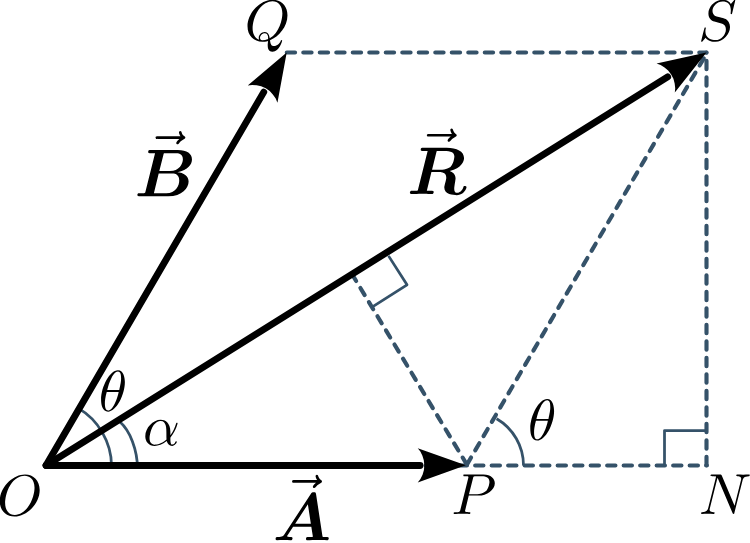
\includegraphics[width=0.3\textwidth]{figures/fig_vec-sum-mag.png}
				\caption{Magnitude of a vector sum}
				\label{fig:vec-sum-mag}
			\end{figure}
			Consider the construction as given in figure \ref{fig:vec-sum-mag}. Because now that $OPSQ$ is a parallelogram, we have
			\begin{align*}
				OP=QS&=|\va*{A}|=A \\
				OQ=SP&=|\va*{B}|=B \\
				\qq{and}OS&=|\va*{R}|=R
			\end{align*}
			Let $\theta$ be the angle between vectors $\va*{A}$ and $\va*{B}$. Then we have $\angle{SPN}=\theta$. Hence, from $\triangle{PSN}$, we obtain
			\begin{align*}
				PN=SP\cos{\theta}&=B\cos{\theta} \\
				\qq{and}SN=SP\sin{\theta}&=B\sin{\theta}
			\end{align*}
			Then in $\triangle{OSN}$, using Pythagoras' theorem, we get
			\begin{align*}
				OS^2&=ON^2+SN^2 \\
				\implies OS^2&=\qty(OP+PN)^2+SN^2 \\
				\implies R^2&=\qty(A+B\cos{\theta})^2+\qty(B\sin{\theta})^2 \\
				&=A^2+B^2\cos^2{\theta}+2AB\cos{\theta}+B^2\sin^2{\theta} \\
				&=A^2+B^2\qty(\cos^2{\theta}+\sin^2{\theta})+2AB\cos{\theta} \\
				\implies R^2&=A^2+B^2+2AB\cos{\theta}
			\end{align*}
			Therefore,
			\begin{align*}
				\Aboxed{|\va*{A}+\va*{B}|=\sqrt{A^2+B^2+2AB\cos{\theta}}}
			\end{align*}
			
		\subsubsection{Direction of the vector sum}
			Let $\alpha$ be the angle between the resultant vector $\va*{R}=\va*{A}+\va*{B}$. Because direction of the vector $\va*{A}$ is already known, knowing the angle $\alpha$ would enable us to know the direction of $\va*{R}$ with respect to $\va*{A}$.
			
			From $\triangle{OSN}$, we obtain,
			\begin{align*}
				\tan{\alpha}&=\dfrac{SN}{ON} \\
				&=\dfrac{SN}{OP+PN} \\
				\implies\tan{\alpha}&=\dfrac{B\sin{\theta}}{A+B\cos{\theta}}
			\end{align*}
			
			Therefore,
			\begin{align*}
				\Aboxed{\alpha=\tan^{-1}{\qty(\dfrac{B\sin{\theta}}{A+B\cos{\theta}})}}
			\end{align*}
			
		\subsubsection{Subtraction on vectors}
			The subtraction of a vector from another may be defined in terms of the addition of one vector with the negative of the other vector, i.e.
			$$\va*{A}-\va*{B}=\va*{A}+\qty(-\va*{B})$$
			The magnitude of the vector difference is:
			\begin{align*}
				\Aboxed{|\va*{A}-\va*{B}|=\sqrt{A^2+B^2-2AB\cos{\theta}}}
			\end{align*}
			
		\subsubsection{Resolution of vectors}
			Suppose we have a certain vector $\va*{A}$ and two arbitrary vectors $\va*{x}$ and $\va*{y}$, all of them being coplanar. Let us now perform the following geometrical constructions.
			\begin{figure}[h!]
				\centering
				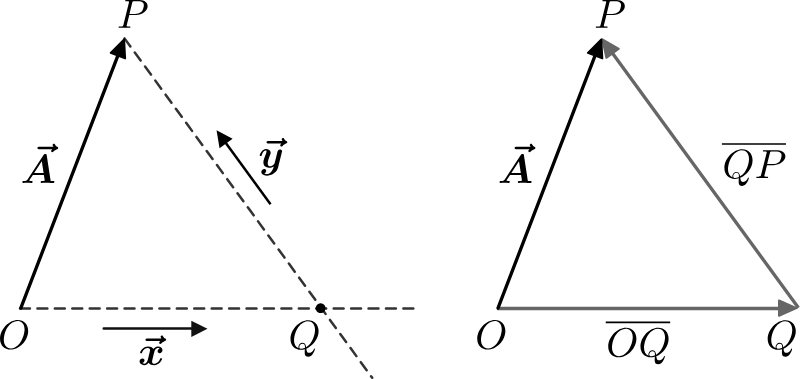
\includegraphics[width=0.5\textwidth]{figures/fig_vec-resolution.png}
			\end{figure}
			\begin{enumerate}[I.]
				\item Through the origin $O$ of vector $\va*{A}$, we draw a straight line parallel to $\va*{x}$.
				\item Through the terminus $P$ of vector $\va*{A}$, we draw another straight line parallel to $\va*{y}$.
				\item Let the point of intersection of these two straight lines be $Q$.
				\item We define the following two vectors:
				\begin{align*}
					\overline{OQ}&:\qq{origin at $O$, terminus at $Q$} \\
					\overline{QP}&:\qq{origin at $Q$, terminus at $P$}
				\end{align*}
			\end{enumerate}
			Then, by triangle law of vector addition, we have
			\begin{align}
				\va*{A}=\overline{OQ}+\overline{QP} \label{eqn:vec-resolution-01}
			\end{align}
			We know that when a vector is multiplied by some scalar, we obtain another parallel vector with different magnitude. Conversely, for two parallel vectors, one of them can be expressed as a scalar multiple of the other.
			
			Consequently, because $\overline{OQ}$ is parallel to $\va*{x}$, we have
			\begin{align}
				\overline{OQ}=\alpha\va*{x} \label{eqn:vec-resolution-02}
			\end{align}
			Also, because $\overline{QP}$ is parallel to $\va*{y}$, we have
			\begin{align}
				\overline{QP}=\beta\va*{y} \label{eqn:vec-resolution-03}
			\end{align}
			where $\alpha$, $\beta$ are some arbitrary constant scalars.
			
			Using equations (\ref{eqn:vec-resolution-02}) and (\ref{eqn:vec-resolution-03}) in equation (\ref{eqn:vec-resolution-01}) gives
			\begin{align}
				\va*{A}=\alpha\va*{x}+\beta\va*{y} \label{eqn:vec-resolution-04}
			\end{align}
			Therefore, equation (\ref{eqn:vec-resolution-04}) shows that given some specific vector, it can be expressed as a vector sum of two arbitrary vectors, with each being multiplied by some constant scalars, and all of them lying on a plane.
			
			Then we may say that the given vector has been resolved along two arbitrary vectors on the same plane, and the procedure followed to do so is known as the \emph{resolution of a vector}.
			
	\subsection{Multiplication of vectors}
	
		\subsubsection{Scalar product (or dot product)}
			Given two vectors $\va*{A}$ and $\va*{B}$ which have an angle $\theta$ between them, their scalar product is a scalar quantity which equals the product of their magnitudes and the cosine of the angle between them.
			
			It is expressed mathematically as
			\begin{align*}
				\va*{A}\vdot\va*{B}&=|\va*{A}||\va*{B}|\cos{\theta} \\
				\qq{or,}\Aboxed{\va*{A}\vdot\va*{B}&=AB\cos{\theta}}
			\end{align*}
			where $A=|\va*{A}|$ and $B=|\va*{B}|$.
			
			Some of the properties of the dot product are:
			\begin{enumerate}
				\item \textit{Commutativity}: The order of vectors does not matter, i.e.
				$$\va*{A}\cdot\va*{B}=\va*{B}\cdot\va*{A}$$
				
				\item \textit{Distributivity}: The scalar product distributes over vector addition, i.e.
				$$\va*{A}\cdot\qty(\va*{B}+\va*{C})=\va*{A}\cdot\va*{B}+\va*{A}\cdot\va*{C}$$
				
				\item The scalar product of a vector with itself equals the square of its magnitude, i.e.
				$$\va*{A}\cdot\va*{A}=A^2$$
				
				\item Multiplying either of the vectors by a scalar affects the scalar product by the same factor, i.e.
				$$\qty(\lambda\va*{A})\cdot\va*{B}=\va*{A}\cdot\qty(\lambda\va*{B})=\lambda\qty(\va*{A}\cdot\va*{B})$$
			\end{enumerate}
			
		\subsubsection{Vector product (or cross product)}
			Given two vectors $\va*{A}$ and $\va*{B}$ which have an angle $\theta$ between them, their vector product is another vector quantity which is perpendicular to the plane that contains both $\va*{A}$ and $\va*{B}$, and is denoted by $\va*{A}\cross\va*{B}$.
			\renewcommand\labelitemi{--}
			\begin{itemize}
				\item The magnitude of $\va*{A}\cross\va*{B}$ is obtained as
				\begin{align*}
					|\va*{A}\cross\va*{B}|=AB\sin{\theta}
				\end{align*}
				
				\item The direction of $\va*{A}\cross\va*{B}$ is obtained using the right-hand thumb rule, which is applied as follows:
				
				\begin{quote}
					If the fingers of one's right hand are curled from the first vector to the second, then the stretched thumb of the right hand points in the direction of their cross product.
				\end{quote}
				
				\item The vector product is anti-commutative, i.e.
				\begin{align*}
					\va*{A}\cross\va*{B}=-\va*{B}\cross\va*{A}
				\end{align*}
				
				Because $\va*{A}\cross\va*{B}$ and $\va*{B}\cross\va*{A}$ are negatives of each other, the order of the cross product is important.
			\end{itemize}
			
			Some of the properties of the cross product are:
			\begin{enumerate}
				\item \emph{Anti-commutativity}: The order of vectors is important, and reversing it changes the direction of the vector product, i.e.
				$$\va*{A}\cross\va*{B}=-\va*{B}\cross\va*{A}$$
				
				\item \emph{Perpendicularity}: The resultant vector product is perpendicular to the plane containing the original vectors.
				
				\item \emph{Magnitude}: The magnitude of the vector product is the area of the parallelogram formed by the two vectors.
				
				\item \textit{Distributivity}: The vector product distributes over vector addition, i.e.
				$$\va*{A}\cross\qty(\va*{B}+\va*{C})=\va*{A}\cross\va*{B}+\va*{A}\cross\va*{C}$$
			\end{enumerate}
			
		\subsubsection{Scalar triple product}
			Given three vectors $\va*{A}$, $\va*{B}$ and $\va*{C}$, their scalar triple product is given as
			\begin{align*}
				[\va*{A}\va*{B}\va*{C}]&=\va*{A}\cdot\qty(\va*{B}\cross\va*{C})
			\end{align*}
			It is calculated as the determinant of a $3\times 3$ matrix formed by the component vectors, with a result of zero indicating the vectors are coplanar.
			
			\renewcommand\labelitemi{--}
			\begin{itemize}
				\item The operation combines a dot product and a cross product acting on three vectors to produce a scalar quantity.
			\end{itemize}